%+++++++++++++++++++++++++++++++++++++++++++++++++++++++++++++++
% SUMMARY    : Lecture 8 
%            : University of Southern Maine 
%            : @james.quinlan
%            : Anusha Ghimire - Lecture 8
%+++++++++++++++++++++++++++++++++++++++++++++++++++++++++++++++
%+++++++++++++++++++++++++++++++++++++++++++++++++++++++++++++++
% SUMMARY    : The Perceptron , Hyperplane, Perceptron Algorithm, Definitions 
%              and Assumptions for model, Classifier equation, Class Code
%            : University of Southern Maine 
%            : @james.quinlan
%            : Anusha Ghimire - Lecture 8
%+++++++++++++++++++++++++++++++++++++++++++++++++++++++++++++++
\section*{Objectives}
\begin{outline}
    \1 The Perceptron 
    \1 Hyperplane
    \1 Perceptron Algorithm
    \1 Definitions and Assumptions for model
    \1 Classifier equation
    \1 Class Code
\end{outline}

\rule[0.0051in]{\textwidth}{0.00025in}
% ----------------------------------------------------------------

\section{The Perceptron}

A perceptron is one of the simplest types of artificial neural network and is a foundational concept in machine learning. 
It is mainly used for binary classification tasks. Introduced by Frank Rosenblatt in 1958, it is one of the earliest neural network models designed to mimic the way the human brain processes information.

The perceptron takes multiple inputs (features), each associated with a weight, and computes a weighted sum. 
This sum is then passed through an activation function, which produces the final output. 
To visualize this, consider a perceptron with four inputs \( x_1, x_2, x_3, x_4 \), each with corresponding weights \( w_1, w_2, w_3, w_4 \), and a bias term \( b \) as shown below.

\begin{center}
\resizebox{!}{5cm}{ % Adjust height, width auto-scales
    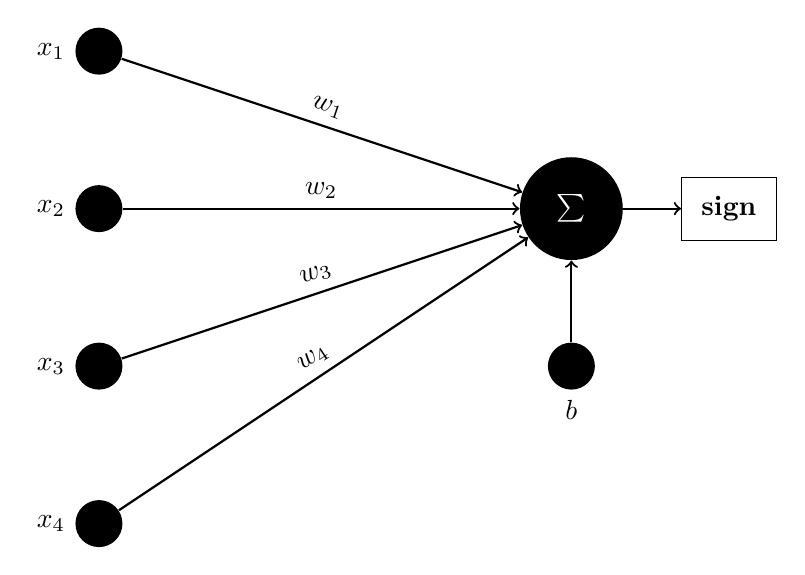
\begin{tikzpicture}
        % Input nodes (features)
        \node[circle, fill=black, inner sep=6pt, label=left:{$x_1$}] (x1) at (0,6) {};
        \node[circle, fill=black, inner sep=6pt, label=left:{$x_2$}] (x2) at (0,4) {};
        \node[circle, fill=black, inner sep=6pt, label=left:{$x_3$}] (x3) at (0,2) {};
        \node[circle, fill=black, inner sep=6pt, label=left:{$x_4$}] (x4) at (0,0) {};

        % Output node (Summation)
        \node[circle, fill=black, inner sep=8pt, text=white] (output) at (6,4) {\Large $\sum$};

        % Bias node
        \node[circle, fill=black, inner sep=6pt, label=below:{$b$}] (bias) at (6,2) {};

        % Activation function (Sign function)
        \node[draw, rectangle, fill=white, minimum width=1.2cm, minimum height=0.8cm] (activation) at (8,4) {\textbf{sign}};

        % Weights and connections
        \draw[thick, ->] (x1) -- node[midway, above, sloped] {\(w_1\)} (output);
        \draw[thick, ->] (x2) -- node[midway, above, sloped] {\(w_2\)} (output);
        \draw[thick, ->] (x3) -- node[midway, above, sloped] {\(w_3\)} (output);
        \draw[thick, ->] (x4) -- node[midway, above, sloped] {\(w_4\)} (output);
        \draw[thick, ->] (bias) -- (output);  % Bias input perpendicular

        % Connection from summation to activation function
        \draw[thick, ->] (output) -- (activation);

    \end{tikzpicture}
}
\end{center}

To make the perceptron useful for real-world classification tasks, it must learn the appropriate weights and bias through training. 
The training process involves adjusting these parameters based on labeled examples.

A training data set consists of multiple examples, where each input \( x_i \) is a \( p \)-dimensional vector representing features, 
and each corresponding label \( y_i \) is either \( -1 \) or \( 1 \) (for binary classification). Formally, we define the training data as follows:

\[
\text{Training Data} = \{(x_1, y_1), (x_2, y_2), \dots, (x_n, y_n)\}
\]

where:

\begin{itemize}
    \item \( x_i \in \mathbb{R}^p \) represents a feature vector with dimensions \( p \).
    \item \( y_i \in \{-1, 1\} \) is the class label that indicates the input category.
\end{itemize}

This data set helps update the weights of the perceptron using a learning algorithm, ensuring that the model can make accurate predictions on unseen data.

% -----------------------------------------------------------------------------------------------

\section{Hyperplane}

A hyperplane is a decision boundary that separates data points into different classes. In binary classification, the hyperplane divides the space into two regions: 
one for positive class (+1) and one for negative class (-1). The hyperplane is represented by a slanted decision boundary that separates the two classes, as shown below. 

\begin{center}
\resizebox{!}{8cm}{ % Adjust height to 8cm, width auto-scales
    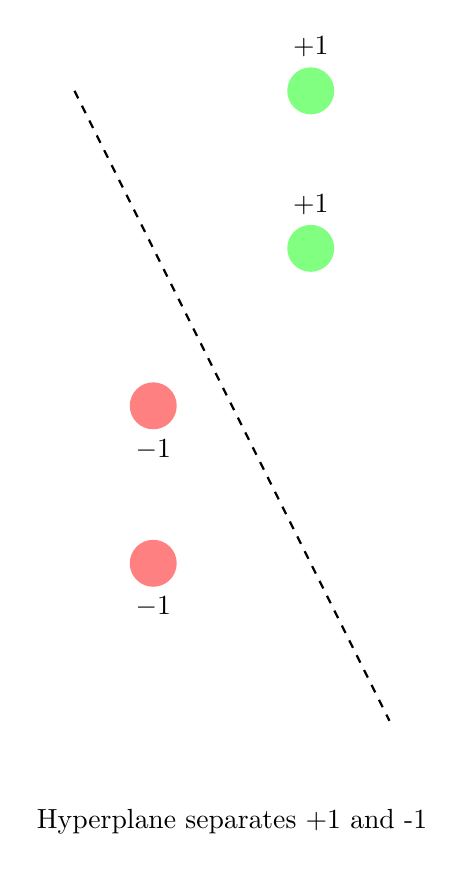
\begin{tikzpicture}
        % Input nodes (features)
        \node[circle, fill=green!50, inner sep=6pt, label=above:{$+1$}] (x1) at (1, 4) {};
        \node[circle, fill=green!50, inner sep=6pt, label=above:{$+1$}] (x2) at (1, 2) {};
        \node[circle, fill=red!50, inner sep=6pt, label=below:{$-1$}] (x3) at (-1, 0) {};
        \node[circle, fill=red!50, inner sep=6pt, label=below:{$-1$}] (x4) at (-1, -2) {};

        % Slanted hyperplane
        \draw[thick, dashed] (-2,4) -- (2,-4);

        % Labels and title
        \node[below] at (0,-5) {Hyperplane separates +1 and -1};
    \end{tikzpicture}
}
\end{center}

When data points are linearly separable, there can be infinitely many hyperplanes that separate the points. These hyperplanes differ in orientation and position, but they all separate the points correctly. The ideal hyperplane is the one that maximizes the margin between the two classes.

\begin{center}
\resizebox{!}{6cm}{ % Adjust height, width auto-scales
    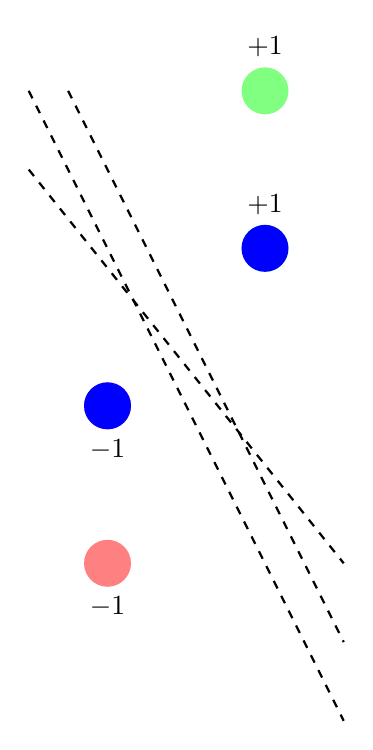
\begin{tikzpicture}
        % Input nodes (features)
        \node[circle, fill=green!50, inner sep=6pt, label=above:{$+1$}] (x1) at (1, 4) {};
        \node[circle, fill=green!50, inner sep=6pt, label=above:{$+1$}] (x2) at (1, 2) {};
        \node[circle, fill=red!50, inner sep=6pt, label=below:{$-1$}] (x3) at (-1, 0) {};
        \node[circle, fill=red!50, inner sep=6pt, label=below:{$-1$}] (x4) at (-1, -2) {};

        % Slanted hyperplanes
        \draw[thick, dashed] (-2,4) -- (2,-4);  % Hyperplane 1
        \draw[thick, dashed] (-1.5,4) -- (2,-3);  % Hyperplane 2
        \draw[thick, dashed] (-2,3) -- (2,-2);  % Hyperplane 3
        
        % Support vectors (marked)
        \node[circle, fill=blue, inner sep=6pt] (s1) at (1,2) {};
        \node[circle, fill=blue, inner sep=6pt] (s2) at (-1,0) {};
    \end{tikzpicture}
}
\end{center}

\subsection{For Different Dimensions}

\begin{itemize}
    \item \textbf{1D }: The hyperplane is just a single point.
    \item \textbf{2D }: The hyperplane is a line that separates the 2D plane.
    \item \textbf{3D }: The hyperplane is a plane that separates the 3D space.
\end{itemize}

\subsection{Mathematical Definition of a Hyperplane}

A hyperplane is a set of vectors \(\mathcal{H}\) such that:

\[
\mathcal{H} = \{ \mathbf{x} \ | \ \mathbf{w}^T \mathbf{x} + b = 0 \}
\]

Where:
\(\mathbf{x} \in \mathbb{R}^p\) is a vector in \(p\)-dimensional space,
\(\mathbf{w}\) is the normal vector to the hyperplane,
\(b\) is the bias term.

The equation represents all the points \(\mathbf{x}\) that lie on the hyperplane.

Thus, there are infinitely many possible hyperplanes that can separate the data points, but the \textbf{maximum margin} hyperplane is the one that best generalizes the decision boundary and is selected by techniques such as Support Vector Machines (SVMs).
\section{Bundle \& Save}

In the hyperplane equation:
\[
w^T x + b = 0
\]
we can bundle the bias term \( b \) as part of the input feature vector by augmenting it with a constant value. Specifically, we define the augmented feature vector:
\[
x' = \begin{bmatrix} x \\ 1 \end{bmatrix}
\]
and the extended weight vector:
\[
w' = \begin{bmatrix} w \\ b \end{bmatrix}
\]
Now the hyperplane equation becomes:
\[
w'^T x' = 0
\]

\section{Assumptions for the Perceptron Model}

Data is Linearly Separable
The data must be \textbf{linearly separable} for the perceptron model to work. This means that a linear hyperplane exists that can perfectly separate the data points belonging to different classes. 

\subsection{What is Linearly Separable?}
For a dataset with inputs \( x_i \) and corresponding labels \( y_i \), where \( y_i \in \{-1, 1\} \), the data is said to be linearly separable if there exists a hyperplane represented by the equation \( w^T x + b = 0 \) such that for each data point:
\[
y_i (w^T x_i + b) > 0
\]
If \( x \) is negative, we take \( y = -1 \), making the equation \( w^T x + b > 0 \).  
If \( x \) is positive, we take \( y = +1 \), which also makes \( w^T x + b > 0 \).


\section{Perceptron Algorithm}

The goal of training a perceptron is to find the optimal weight vector \( \mathbf{w} \) and bias \( b \) such that the perceptron can correctly classify the input data.

The perceptron makes predictions using the following equation:
\[
\hat{y} = \text{sign}(\mathbf{w}^T \mathbf{x} + b)
\]
Where:
 \( \mathbf{w} \) is the weight vector,
 \( \mathbf{x} \) is the input feature vector,
 \( b \) is the bias term, and
 \( \hat{y} \) is the predicted label (+1 or -1).

\subsection{Goal of Training}
The objective of perceptron training is to find the optimal weight vector \( \mathbf{w} \) and bias \( b \) that minimize classification errors on the training set. 

\section{Exercise: Check if \( \mathbf{u} = [3, -2, 1]^T \) belongs to the hyperplane}

We are given:
\[
\mathbf{w} = \begin{bmatrix} 1 \\ 2 \\ -3 \end{bmatrix}, \quad b = 4, \quad \mathbf{u} = \begin{bmatrix} 3 \\ -2 \\ 1 \end{bmatrix}
\]
We need to check if \( \mathbf{u} \) lies on the hyperplane defined by the equation:
\[
\mathbf{w}^T \mathbf{u} + b = 0
\]
Substitute the values into the equation:
\[
\mathbf{w}^T \mathbf{u} + b = 1(3) + 2(-2) + (-3)(1) + 4
\]
\[
= 3 - 4 - 3 + 4 = 0
\]
Since the result is \( 0 \), this means that \( \mathbf{u} = [3, -2, 1]^T \) lies on the hyperplane \( \mathcal{H} \).


\subsection{Why is \( \mathbf{w} \) Perpendicular?}
\begin{itemize}
    \item For any point \( \mathbf{x}_0 \) on the hyperplane, it satisfies the equation \( \mathbf{w}^T \mathbf{x}_0 + b = 0 \).
    \item Now, if you take any vector \( \mathbf{v} \) that lies on the hyperplane (i.e., any vector \( \mathbf{v} \) such that the line formed by \( \mathbf{x}_0 + \mathbf{v} \) also lies on the hyperplane), the following condition must hold:
    \[
    \mathbf{w}^T (\mathbf{x}_0 + \mathbf{v}) + b = 0
    \]
    Since \( \mathbf{x}_0 \) lies on the hyperplane, \( \mathbf{w}^T \mathbf{x}_0 + b = 0 \). Therefore, the equation simplifies to:
    \[
    \mathbf{w}^T \mathbf{v} = 0
    \]
    This means that \( \mathbf{w} \) is perpendicular to \( \mathbf{v} \), as \( \mathbf{v} \) lies on the hyperplane. Hence, \( \mathbf{w} \) is perpendicular to every vector on the hyperplane.
\end{itemize}

\section{Classifier Equation}


The general form of the classifier is:
\[
h(x) = \text{sign}(\mathbf{w}^T \mathbf{x} + b)
\]
Where:
\( \mathbf{x} \) is the input feature vector,
\( \mathbf{w} \) is the weight vector,
\( b \) is the bias term,
\( \text{sign}(\cdot) \) is the sign function, which outputs \( +1 \) if the input is positive and \( -1 \) if the input is negative.

\begin{itemize}
    \item \textbf{Algorithm Finds \( \mathbf{w} \) and \( b \) Based on Training Data:} 
    During the training phase, the algorithm adjusts the weight vector \( \mathbf{w} \) and bias \( b \) based on the labeled training data. 
    The goal is to find values for \( \mathbf{w} \) and \( b \) that minimize classification errors and effectively separate the data points into their respective classes. 
    The training process involves optimizing the parameters based on the data's features and labels.

    \item \textbf{Classifying New Data:} 
    For new, unseen data, the classifier uses the learned values of \( \mathbf{w} \) and \( b \) to make a prediction. 
    The new data point \( \mathbf{x} \) is classified by evaluating the equation:
    \[
    h(x) = \text{sign}(\mathbf{w}^T \mathbf{x} + b)
    \]
    \begin{itemize}
        \item If \( \mathbf{w}^T \mathbf{x} + b > 0 \), then the classifier predicts class \( +1 \).
        \item If \( \mathbf{w}^T \mathbf{x} + b < 0 \), then the classifier predicts class \( -1 \).
    \end{itemize}
\end{itemize}

\section{Class Code(Perceptron Algorithm Steps)}

\begin{itemize}
    \item \textbf{Input:} A dataset \( D = \{(x_1, y_1), (x_2, y_2), \dots, (x_n, y_n)\} \), where \( x_i \) is the feature vector and \( y_i \in \{-1, 1\} \) is the label for each data point.
    \item \textbf{Output:} The learned weight vector \( w \) and bias \( b \).
    \item \textbf{Initialize:} 
    \[
    w = \mathbf{0} \quad \text{(weight vector initialized to zero)}, \quad b = 0 \quad \text{(bias initialized to zero)}.
    \]
    \item \textbf{Algorithm Steps:}
    \begin{enumerate}
        \item Set \( m = 1 \) (initially assuming there are misclassifications).
        \item \text{While } \( m > 0 \) \text{ (until no misclassifications)}:
        \begin{enumerate}
            \item Set \( m = 0 \) (assume no misclassifications for this iteration).
            \item For each data point \( i = 1 \) to \( n \):
            \begin{itemize}
                \item If \( y_i (w^T x_i + b) \leq 0 \) (the point is misclassified):
                \item Update the weight vector: 
                \[
                w = w + y_i x_i
                \]
                \item Increment the misclassification count: \( m = m + 1 \)
            \end{itemize}
        \end{enumerate}
    \end{enumerate}
\end{itemize}
\end{minted}
